\chapter{Integration of the Equations of Motion}

% ============ Problem 1 ============ %

\begin{problem}
{
Determine the period of oscillations of a simple pendulum (a particle of mass $m$ suspended by a string of length $l$ in a gravitational field) as a function of the amplitude of the oscillations.
}
{
The potential energy of a simple pendulum is
\begin{equation*}
   U(\phi) = - mgl\cos{\phi},
\end{equation*}
see \probref{1}{1}. If we define $\phi_0$ as the maximum value of $\phi$, the potential energy is equal to the total energy at this point, that is
\begin{equation*}
    U(\phi_0) = E = -mgl\cos{\phi_0}.
\end{equation*}
The energy of the pendulum could also be write using the kinetic energy,
\begin{equation*}
    E = \frac{1}{2}ml^2\Dot{\phi}^2 + U(\phi).
\end{equation*}
This first order differential equation can be integrate to give the the period of oscillation 
\begin{align*}
    T &= 2\sqrt{\frac{ml^2}{2}} \int_{-\phi_0}^{\phi_0} \frac{d\phi}{\sqrt{E-U(\phi)}} \\
    &= 4\sqrt{\frac{ml^2}{2}} \int_{0}^{\phi_0} \frac{d\phi}{\sqrt{mgl\cos{\phi}-mgl\cos{\phi_0}}} \\
    &= 4\sqrt{\frac{l}{2g}} \int_{0}^{\phi_0} \frac{d\phi}{\sqrt{\cos{\phi}-\cos{\phi_0}}}.
\end{align*}
To solve this integral, we need first to use a trigonometric identity (I'll let you find or derive this identity), giving us
\begin{equation*}
    T = 2\sqrt{\frac{l}{g}} \int_{0}^{\phi_0} \frac{d\phi}{\sqrt{\sin^2{\frac{\phi_0}{2}}-\sin^2{\frac{\phi}{2}}}}.
\end{equation*}
Next, we use the substitution
\begin{equation*}
    \sin{\xi} = \frac{\sin{\frac{\phi}{2}}}{\sin{\frac{\phi_0}{2}}}.
\end{equation*}
It's differential form is
\begin{align*}
    \frac{d\phi}{d\xi} &= \frac{d}{d\xi} \left( 2 \arcsin{\left(\sin{\frac{\phi_0}{2}}\sin{\xi}\right)} \right) \\
    &= \frac{2\sin{\frac{\phi_0}{2}}\cos{\xi}}{\sqrt{1-\sin^2{\frac{\phi_0}{2}}\sin^2{\xi}}}
\end{align*}
The substitution, finally, give
\begin{align*}
    T &= 2\sqrt{\frac{l}{g}} \int_{0}^{\phi_0} \frac{d\phi}{\sqrt{\sin^2{\frac{\phi_0}{2}} - \sin^2{\xi}\sin^2{\frac{\phi_0}{2}}}} \\
    &= 2\sqrt{\frac{l}{g}} \int_{0}^{\phi_0} \frac{d\phi}{\sin{\frac{\phi_0}{2}}\sqrt{ 1 - \sin^2{\xi}}} \\
    &= 2\sqrt{\frac{l}{g}} \int_{0}^{\phi_0} \frac{d\phi}{\sin{\frac{\phi_0}{2}}\cos{\xi}} \\
    &= 2\sqrt{\frac{l}{g}} \int_{\arcsin{(0)}}^{\arcsin{(1)}} \frac{2\sin{\frac{\phi_0}{2}}\cos{\xi} d\xi}{\sin{\frac{\phi_0}{2}}\cos{\xi}\sqrt{1-\sin^2{\frac{\phi_0}{2}}\sin^2{\xi}}} \\
    &= 4\sqrt{\frac{l}{g}} \int_{0}^{\frac{\pi}{2}} \frac{d\xi}{\sqrt{1-\sin^2{\frac{\phi_0}{2}}\sin^2{\xi}}}.
\end{align*}
We can also write
\begin{equation*}
    T = 4\sqrt{\frac{l}{g}} K\left(\sin{\frac{\phi_0}{2}}\right),
\end{equation*}
where 
\begin{equation} \label{C3P1_K}
    K(k) = \int_{0}^{\frac{\pi}{2}} \frac{d\xi}{\sqrt{1-k\sin^2{\xi}}}.
\end{equation}
The integral $K$ is known as the complete elliptic integral of the first kind. To solve this integral, we first need to see that the integrand is of the form 
\begin{equation*}
    f(x) = \left( 1 - x \right)^{-\frac{1}{2}}.
\end{equation*}
The $n$ derivative of this function is
\begin{equation*}
    f^{(n)}(x) = \frac{\left( 2n-1 \right)!!}{2^n}\left( 1-x \right)^{\frac{-2n+1}{2}},
\end{equation*}
thus the Maclaurin Series is
\begin{equation*}
    f(x) = \sum_{n\geq0}\frac{(2n-1)!!}{2^n \cdot n!}x^n.
\end{equation*}
Using this result in \eqref{C3P1_K}, we get
\begin{align*}
    K(k) &= \int_{0}^{\frac{\pi}{2}} \sum_{n\geq0}\frac{(2n-1)!!}{2^n \cdot n!}k^{2n}\sin^{2n}{\xi}\;d\xi \\
    &= \sum_{n\geq0}\frac{(2n-1)!!}{2^n \cdot n!}k^{2n} \int_{0}^{\frac{\pi}{2}} \sin^{2n}{\xi}\;d\xi.
\end{align*}
This last integral can be solve using the beta function
\begin{equation*}
    \mathcal{B}(x,y) = \frac{\Gamma(x)\Gamma(y)}{\Gamma(x+y)} = 2\int_0^{\frac{\pi}{2}} \sin^{2x-1}{t}\cos^{2y-1}{t}\;dt,
\end{equation*}
with $x=\frac{2n+1}{2}$ and $y=\frac{1}{2}$. Thus, the beta function become
\begin{align*}
    \frac{1}{2}\mathcal{B}(x,y) &= \frac{\Gamma(x)\Gamma(y)}{2\Gamma(x+y)} \\
    &= \frac{\sqrt{\pi}}{2}\frac{\Gamma(\frac{2n+1}{2})}{n!} \\
    &= \frac{\pi}{2}\frac{(2n+1)!!}{2^n \cdot n!}
\end{align*}
The elliptic integral is thereby
\begin{align*}
    K(k) &= \frac{\pi}{2} \sum_{n\geq0}\left[\frac{(2n-1)!!}{2^n \cdot n!}k^{n}\right]^2 \\
    &= \frac{\pi}{2} \sum_{n\geq0}\left[\frac{(2n-1)!!}{(2n)!!}k^{n}\right]^2.
\end{align*}
The period of a simple pendulum is
\begin{equation*}
    T = 2\pi\sqrt{\frac{l}{g}}\sum_{n\geq0}\left[\frac{(2n-1)!!}{(2n)!!}\sin^n{\frac{\phi_0}{2}}\right]^2
\end{equation*}
By expanding the sum, we get
\begin{equation*}
    T = 2\pi\sqrt{\frac{l}{g}}\left( 1 + \left(\frac{1}{2}\right)^2\sin^2{\frac{\phi}{2}} + \left(\frac{1\cdot3}{2\cdot4}\right)^2\sin^4{\frac{\phi}{2}} + \left(\frac{1\cdot3\cdot5}{2\cdot4\cdot6}\right)^2\sin^6{\frac{\phi}{2}} + \ldots \right).
\end{equation*}
Using the Maclaurin series
\begin{equation*}
    \sin{\frac{\phi_0}{2}} = \frac{1}{2}\phi_0 - \frac{1}{48}\phi_0^3 + \frac{1}{3840}\phi_0^5 - \frac{1}{645120}\phi_0^7 + \ldots,
\end{equation*}
we finally get
}
{
\begin{equation*}
    T = 2\pi\sqrt{\frac{l}{g}}\left( 1 + \frac{1}{16}\phi_0^2 + \frac{11}{3072}\phi_0^4 + \ldots \right)
\end{equation*}
}
\end{problem}

% ============ Problem 2 ============ %

\begin{problem}
{
Determine the period of oscillation, as a function of the energy, when a particle of mass $m$ moves in fields for which the potential energy is
}{}{}
\end{problem}
\begin{subproblem}
{
\begin{equation*}
    U = A|x|^n
\end{equation*}
}
{
The total energy of the particle is
\begin{equation*}
    E = \frac{1}{2}m\Dot{x}^2 + U(x).
\end{equation*}
Knowing that the maximum value of $E$ is at $x_1$, this position is
\begin{align*}
    &E = U(x_1) = A|x_1|^n \\
    \Rightarrow &|x_1| = \left( \frac{E}{A} \right)^{1/n}, \\
     \Rightarrow &x_1 = \pm \left( \frac{E}{A} \right)^{1/n},
\end{align*}
we get the period of oscillation,
\begin{align*}
    T &= 2\sqrt{\frac{m}{2}} \int_{-\left( \frac{E}{A} \right)^{1/n}}^{\left( \frac{E}{A}\right)^{1/n} }\frac{dx}{\sqrt{E-A|x|^n}} \\
    &= 2\sqrt{2m} \int_0^{\left( \frac{E}{A}\right)^{1/n} }\frac{dx}{\sqrt{E-A|x|^n}} .
\end{align*}
It is possible to remove the absolute value, because the integral is over positive $x$, thus
\begin{align*}
    T &= 2\sqrt{2m} \int_0^{\left( \frac{E}{A}\right)^{1/n} }\frac{dx}{\sqrt{E-Ax^n}} \\
    &= 2\sqrt{\frac{2m}{E}} \int_0^{\left( \frac{E}{A}\right)^{1/n} }\frac{dx}{\sqrt{1-\frac{A}{E}x^n}}.
\end{align*}
Using the substitution $y = \left(\frac{A}{E}\right)^{\frac{1}{n}}x$, we get
\begin{align*}
    T &= 2\sqrt{\frac{2m}{E}} \int_0^1 \frac{\left(\frac{A}{E}\right)^{\frac{1}{n}}dy}{\sqrt{1-\frac{A}{E}\left(\left(\frac{A}{E}\right)^{\frac{-1}{n}}y\right)^n}} \\
    &= 2\sqrt{\frac{2m}{E}} \left(\frac{E}{A}\right)^{\frac{1}{n}} \int_0^1 \frac{dy}{\sqrt{1-y^n}} .
\end{align*}
Using another substitution $u = y^n$, we get
\begin{equation*}
    T = 2\sqrt{\frac{2m}{E}} \left(\frac{E}{A}\right)^{\frac{1}{n}} \int_0^1 \frac{u^{\frac{1}{n}}du}{nu\sqrt{1-u}} .
\end{equation*}
It is possible to express this integral in term of the beta function
\begin{equation*}
    \mathcal{B}(z_1,z_2) = \int_0^1  t^{z_1-1}\left( 1 - t \right)^{z_2-1}dt = \frac{\Gamma\left(z_1\right)\Gamma\left(z_2\right)}{\Gamma\left(z_1+z_2\right)},
\end{equation*}
with $z_1 = \frac{1}{n}$ and $z_2 = \frac{1}{2}$. This give us
\begin{equation*}
    T = \frac{2}{n}\sqrt{\frac{2m}{E}} \left(\frac{E}{A}\right)^{\frac{1}{n}} \frac{\Gamma\left(\frac{1}{n}\right)\Gamma\left(\frac{1}{2}\right)}{\Gamma\left(\frac{1}{2}+\frac{1}{n}\right)} .
\end{equation*}
Knowing that $\Gamma\left(\frac{1}{2}\right) = \sqrt{\pi}$, we finally have
}
{
\begin{equation*}
    T = \frac{2}{n}\sqrt{\frac{2\pi m }{E}} \left(\frac{E}{A}\right)^{\frac{1}{n}} \frac{\Gamma\left(\frac{1}{n}\right)}{\Gamma\left(\frac{1}{2}+\frac{1}{n}\right)}
\end{equation*}
}
\end{subproblem}

\begin{subproblem}
{
\begin{equation*}
    U = \frac{-U_0}{\cosh^2{\alpha x}}
\end{equation*}
}
{
The two boundaries of the energy are at $E=0 \Rightarrow x=x_1$ and $E=-U_0 \Rightarrow x=0$. The period of oscillation is thus
\begin{align*}
    T &= 2\sqrt{2m} \int_0^{x_1}\frac{dx}{\sqrt{E-U}} \\
    &= 2\sqrt{2m} \int_0^{x_1}\frac{dx}{\sqrt{E+\frac{U_0}{\cosh^2{\alpha x}}}} \\
    &= 2\sqrt{2m} \int_0^{x_1}\frac{\cosh^2{\alpha x} \quad dx}{\sqrt{E\cosh^2{\alpha x}+U_0}}.
\end{align*}
Using the identity $\cosh^2{\alpha x} = 1 + \sinh^2{\alpha x}$, we get
\begin{equation*}
    T = 2\sqrt{2m} \int_0^{x_1}\frac{\cosh^2{\alpha x} \quad dx}{\sqrt{E\left(1+\sinh^2{\alpha x}\right)+U_0}}.
\end{equation*}
The substitution $y=\sinh{\alpha x}$, give us $dy = \alpha\cosh{\alpha x}dx$ and
\begin{align*}
    y(x_1) &= \sinh{\alpha x} \\
    &= \sqrt{\sinh^2{\alpha x}} \\
    &= \sqrt{ \cosh^2{\alpha x} - 1 }\\
    &= \sqrt{\frac{-U_0}{E} - 1}.
\end{align*}
Using this substitution, we get
\begin{align*}
    T &= \frac{2}{\alpha}\sqrt{2m} \int_0^{\sqrt{\frac{-U_0}{E} - 1}} \frac{dy}{E\left( 1 + y^2 \right) + U_0} \\
    &= \frac{2}{\alpha}\sqrt{2m} \int_0^{\sqrt{\frac{-U_0}{E} - 1}} \frac{dy}{E+ Ey^2 - E\cosh^2{\alpha x}}
\end{align*}
Factoring $|E|$ out of the square root (because $E<0$), we have
\begin{align*}
    T &= \frac{2}{\alpha}\sqrt{\frac{2m}{|E|}} \int_0^{\sqrt{\frac{-U_0}{E} - 1}} \frac{dy}{1-\cosh^2{\alpha x} + y^2} \\
    &= \frac{2}{\alpha}\sqrt{\frac{2m}{|E|}} \int_0^{\sqrt{\frac{-U_0}{E} - 1}} \frac{dy}{\sqrt{\frac{-U_0}{E} - 1} + y^2}
\end{align*}
This integral is of the form
\begin{equation*}
    \int_0^a \frac{dz}{\sqrt{a + z^2}} = \sin^{-1}{\left(\frac{z}{a}\right)} = \frac{\pi}{2}.
\end{equation*}
Thus, the period of oscillation is
}
{
\begin{equation*}
    T = \frac{\pi}{\alpha}\sqrt{\frac{2m}{|E|}}
\end{equation*}
}
\end{subproblem}

\begin{subproblem}
{
\begin{equation*}
    U=U_0\tan^2{\alpha x}
\end{equation*}
}
{
The period of oscillation is
\begin{align*}
    T &= 2 \sqrt{2m} \int_0^{x_1} \frac{dx}{\sqrt{E-U}} \\
    &= 2 \sqrt{2m} \int_0^{x_1} \frac{dx}{\sqrt{E-U_0\tan^2{\alpha x}}} \\
    &= 2 \sqrt{2m} \int_0^{x_1} \frac{\cos{\alpha x} \quad dx}{\sqrt{E\cos^2{\alpha x}-U_0\sin^2{\alpha x}}} \\
    &= 2 \sqrt{2m} \int_0^{x_1} \frac{\cos{\alpha x} \quad dx}{\sqrt{E-(E+U_0)\sin^2{\alpha x}}}.
\end{align*}
Using the substitution $y=i\sin{\alpha x}$ $\left(dy = i\alpha\cos{\alpha x}\right)$, we get
\begin{align*}
    T &= \frac{2\sqrt{2m}}{i\alpha} \int_0^{i\sin{\alpha x_1}} \frac{dy}{\sqrt{E+\left( E+U_0 \right)y^2}} \\
    &=  \frac{2}{i\alpha}\sqrt{\frac{2m}{E+U_0}} \int_0^{i\sin{\alpha x_1}} \frac{dy}{\sqrt{\frac{E}{\left( E+U_0 \right)}+y^2}} \\
    &= \frac{2}{i\alpha}\sqrt{\frac{2m}{E+U_0}} \sin^{-1}{\left( \frac{i\sin{\alpha x_1}}{\sqrt{\frac{E}{\left(E+U_0\right)}}} \right)}
\end{align*}
Knowing
\begin{equation*}
    x_1 = \frac{1}{\alpha} \tan^{-1}{\sqrt{\frac{E}{U_0}}},
\end{equation*}
we finally get
\begin{align*}
    T &= \frac{2}{i\alpha}\sqrt{\frac{2m}{E+U_0}} \sin^{-1}{\left( \frac{i\sin{\left(\tan^{-1}{\sqrt{\frac{E}{U_0}}}\right)}}{\sqrt{\frac{E}{\left(E+U_0\right)}}} \right)} \\
    &= \frac{2}{i\alpha}\sqrt{\frac{2m}{E+U_0}} \sin^{-1}{\left( \frac{i\sqrt{\frac{E}{U_0}}}{\sqrt{1+\frac{E}{U_0}}\sqrt{\frac{E}{\left(E+U_0\right)}}} \right)} \\
    &= \frac{2}{i\alpha}\sqrt{\frac{2m}{E+U_0}} \sin^{-1}{i} \\
    &= \frac{2}{i\alpha}\sqrt{\frac{2m}{E+U_0}} \frac{\pi i}{2}.
\end{align*}
Thus, the period of oscillation is
}
{
\begin{equation*}
    T=\frac{\pi}{\alpha}\sqrt{\frac{2m}{E+U_0}}
\end{equation*}
}
\end{subproblem}

% ============ Problem 3 ============ %

\begin{problem}
{
A system consists of one particle of mass $M$ and $n$ particles with equal masses $m$. Eliminate the motion of the centre of mass and so reduce the problem to one involving $n$ particles.
}
{
Let $\mathbf{R}$ be the radius vector of the particle of mass $M$, and $\mathbf{R}_a \left( a=1, 2, \ldots, n \right)$ those of the particles of mass $m$. We put $\mathbf{r}_a \equiv \mathbf{R}_a - \mathbf{R}$ and take the origin to be at the centre of mass, namely
\begin{equation*}
    M\mathbf{R} + m\sum_a \mathbf{R}_a = 0.
\end{equation*}
Thus, we got
\begin{equation} \label{C3P3_R}
    \mathbf{R} = -\frac{m}{M}\left(\sum_a\mathbf{r}_a + n\mathbf{R}\right) = -\frac{m}{\mu} \sum_a \mathbf{r}_a,
\end{equation}
where $\mu \equiv M + nm$. The Lagrangian of the system is
\begin{equation*}
    L = \frac{1}{2}M\Dot{\mathbf{R}}^2 + \frac{1}{2}m\sum_a\Dot{\mathbf{R}}_a^2 - U.
\end{equation*}
If we substitute \eqref{C3P3_R} and $\mathbf{R}_a = \mathbf{R} + \mathbf{r}_a$, we get
\begin{align*}
    L &= \frac{1}{2}\frac{Mm^2}{\mu^2} \left( \sum_a \Dot{\mathbf{r}}_a \right)^2 + \frac{1}{2}nm\Dot{\mathbf{R}}^2 + \frac{1}{2}m\sum_a\Dot{\mathbf{r}}_a^2 + m\Dot{\mathbf{R}}\sum_a \Dot{\mathbf{r}}_a - U \\
    &= \frac{1}{2}\frac{Mm^2}{\mu^2} \left( \sum_a \Dot{\mathbf{r}}_a \right)^2 + \frac{1}{2}\frac{m^3}{\mu^2}\left( \sum_a \Dot{\mathbf{r}}_a \right)^2 + \frac{1}{2}m\sum_a\Dot{\mathbf{r}}_a^2 - \frac{m^2}{\mu}\left(\sum_a \Dot{\mathbf{r}}_a\right)^2 - U \\
    &= \frac{1}{2}m\sum_a\Dot{\mathbf{r}}_a^2 - \frac{1}{2}\frac{m^2}{\mu}\left( \frac{2\mu-M-nm}{\mu} \right)\left(\sum_a \Dot{\mathbf{r}}_a\right)^2.
\end{align*}
The Lagrangian is thus only a function of $\mathbf{r}_a$ and it's time derivative, which is
}
{
\begin{equation*}
    L = \frac{1}{2}m\sum_a\Dot{\mathbf{r}}_a^2 - \frac{1}{2}\frac{m^2}{\mu}\left(\sum_a \Dot{\mathbf{r}}_a\right)^2
\end{equation*}
}
\end{problem}

% ============ Problem 4 ============ %

\begin{problem}
{
Integrate the equations of motion for a spherical pendulum (a particle of mass $m$ moving on the surface of a sphere of radius $l$ in a gravitational field).
\begin{figure}[H]
    \centering
    \includegraphics[page=7]{Figures/tikzpics.pdf}
\end{figure}
}
{
The Cartesian position of the particle $m$ is
\begin{align*}
    x &= l\sin{\theta}\cos{\phi} \\
    y &= l\sin{\theta}\sin{\phi} \\
    z &= -l\cos{\theta}.
\end{align*}
The time derivatives of these coordinates are
\begin{align*}
    \Dot{x} &= l\Dot{\theta}\cos{\theta}\cos{\phi} - l\Dot{\phi}\sin{\theta}\sin{\phi} \\
    \Dot{y} &= l\Dot{\theta}\cos{\theta}\sin{\phi} + l\Dot{\phi}\sin{\theta}\cos{\phi} \\
    \Dot{z} &= l\Dot{\theta}\sin{\theta}.
\end{align*}
Substituting these expressions in the Lagrangian, we obtain the desired Lagrangian form, that is
\begin{align*}
    L &= \frac{1}{2}m\left(\Dot{x}^2+\Dot{y}^2+\Dot{z}^2\right) - mgz \\
    &= \frac{1}{2}ml^2\left(\Dot{\theta}^2+\Dot{\phi}^2\sin^2{\theta}\right) + mgl\cos{\theta}.
\end{align*}
The Lagrangian does not involve $\phi$ explicitly, thus this co-ordinate is cyclic and the generalized momentum $p_\phi$ is conserved. This momentum is the same as the $z$-component of angular momentum $M_z$ and is written
\begin{equation} \label{C3P4_Mz}
    M_z = p_{\phi} = \pd{L}{\Dot{\phi}} = ml^2\Dot{\phi}\sin^2{\theta}.
\end{equation}
The energy of the pendulum is
\begin{equation*}
    E = \frac{1}{2}ml^2\left(\Dot{\theta}^2+\Dot{\phi}^2\sin^2{\theta}\right) - mgl\cos{\theta}.
\end{equation*}
Substituting $\Dot{\phi}$ with \eqref{C3P4_Mz} in the energy we get
\begin{align*}
    E &= \frac{1}{2}ml^2\Dot{\theta}^2 + \frac{M_z^2}{2ml^2\sin^2{\theta}} - mgl\cos{\theta} \\
    &= \frac{1}{2}ml^2\Dot{\theta}^2 + U_{\text{eff}}(\theta),
\end{align*}
where $U_{\text{eff}}(\theta)$ is the effective potential energy. Notice that the energy was re-written as a function of only one co-ordinate (\ie $\theta$). This is equivalent to the one particle problem we have already see, thus
\begin{align*}
    & \frac{d\theta}{dt} = \sqrt{\frac{2\left( E - U_{\text{eff}}(\theta) \right)}{ml^2}} \\
    \Rightarrow & t = \int \frac{d\theta}{\sqrt{2\left( E - U_{\text{eff}}(\theta) \right)}} .
\end{align*}
This integral lead to an elliptic integral of the first kind see \probref{3}{1}. We also need to find the solution to the angle $\phi$. To do so, we can use the \eqref{C3P4_Mz} with the chain rule from calculus, that is
\begin{align*}
    \frac{M_z}{ml^2\sin^2{\theta}} &= \frac{d\phi}{dt} \\
    &= \frac{d\phi}{d\theta}\frac{d\theta}{dt} \\
    &= \frac{d\phi}{d\theta}\sqrt{\frac{2\left( E - U_{\text{eff}}(\theta) \right)}{ml^2}}.
\end{align*}
Finally, we get 
\begin{align*}
    & \frac{d\phi}{d\theta} =  \frac{M_z}{l\sin^2{\theta}} \sqrt{\frac{1}{2m\left( E - U_{\text{eff}}(\theta) \right)}} \\
    \Rightarrow & \phi = \frac{M_z}{l}\sqrt{\frac{1}{2m}}\int\frac{d\theta}{\sin^2{\theta}\left( E - U_{\text{eff}}(\theta) \right)}.
\end{align*}
This integral lead to an elliptic integral of the third kind (I really don't want to solve this). It is possible to find the range of angle $\theta$. At the maximum and minimum value of $\theta$, the pendulum as no kinetic energy, thus
\begin{align*}
    E &= U_{\text{eff}} \\
    &= \frac{M_z^2}{2ml^2\sin^2{\theta}} - mgl\cos{\theta} \\
    &= \frac{M_z^2}{2ml^2\left(1-\cos^2{\theta}\right)} - mgl\cos{\theta}
\end{align*}
We can find a cubic algebraic equation for $\cos{\theta}$, that is
\begin{align*}
    0 &= \left( E + mgl\cos{\theta} \right) \left( 2ml^2 \left( 1 - \cos^2{\theta} \right) \right) - M_z^2 \\
      &= mgl\left(\cos^3{\theta} - \cos{\theta}\right) + E\left(\cos^2{\theta} - 1\right) + \frac{M_z^2}{2ml^2} .
\end{align*}
The centrifugal part of the effective potential $U_{\text{eff}}$, namely
\begin{equation*}
    \frac{M_z^2}{2ml^2\sin^2{\theta}},
\end{equation*}
must be positive. As we can see, this term diverge at $\theta \rightarrow 0$ and $\theta \rightarrow \pi$, thus the angle $\theta$ is bound. This can be write as
\begin{align*}
  \theta &\in \left[ \theta_p, \theta_a\right] & 0 &< \theta_p \leq \theta_a < \pi,
\end{align*}
where the subscripts of the angles $\theta_p$ and $\theta_a$ are for the perigee and apogee. This mean that the two roots of the cubic algebraic equation for $\cos{\theta}$ is bound between $-1$ and $+1$. To summarize, the solution of the equation of motion of the spherical pendulum is
}
{
\begin{align*}
  t &= \int_{\theta_p}^{\theta_a} \frac{d\theta}{\sqrt{2\left( E - U_{\text{eff}}(\theta) \right)}} & \phi &= \frac{M_z}{l}\sqrt{\frac{1}{2m}}\int_{\theta_p}^{\theta_a}\frac{d\theta}{\sin^2{\theta}\left( E - U_{\text{eff}}(\theta) \right)}
\end{align*}
}
\end{problem}

% ============ Problem 5 ============ %

\begin{problem}
{
Integrate the equations of motion for a particle moving on the surface of a cone (of vertical axis $2\alpha$) placed vertically and with vertex downwards in a gravitational field.
}
{
By using the  spherical co-ordinate, we can write the position of the particle as 
\begin{align*}
    x &= r\cos{\phi}\sin{\alpha} \\
    y &= r\sin{\phi}\sin{\alpha} \\
    z &= r\cos{\alpha}.
\end{align*}
By taking the time derivative of those, we obtain
\begin{align*}
    \Dot{x} &= \Dot{r}\cos{\phi}\sin{\alpha} - r\Dot{\phi}\sin{\phi}\sin{\alpha} \\
    \Dot{y} &= \Dot{r}\sin{\phi}\sin{\alpha} + r\Dot{\phi}\cos{\phi}\sin{\alpha} \\
    \Dot{z} &= \Dot{r}\cos{\alpha}.
\end{align*}
The Lagrangian is thus
\begin{align*}
    L &= \frac{1}{2}m\left( \Dot{x}^2 + \Dot{y}^2 + \Dot{z}^2 \right) - mgz \\
    &= \frac{1}{2}m\left( \Dot{r}^2 + r^2\Dot{\phi}^2\sin^2{\alpha} \right) -mgr\cos{\alpha} .
\end{align*}
The co-ordinate $\phi$ is cyclic, thus 
\begin{equation} \label{C3P5_Mz}
    M_z = p_{\phi} = \pd{L}{\Dot{\phi}} = mr^2\Dot{\phi}\sin^2{\alpha}
\end{equation}
is conserved. The energy of the particle is
\begin{equation} \label{C3P5_E}
    E = \frac{1}{2}m\left( \Dot{r}^2 + r^2\Dot{\phi}^2\sin^2{\alpha} \right) + mgr\cos{\alpha} .
\end{equation}
We can rewrite \eqref{C3P5_Mz} as
\begin{equation*}
    \Dot{\phi}^2 =  \frac{M_z^2}{m^2r^4\sin^4{\alpha}}
\end{equation*}
and substituting in \eqref{C3P5_E}, we get
\begin{align*}
    E &= \frac{1}{2}m\Dot{r}^2 + \frac{M_z^2}{2mr^2\sin^2{\alpha}} + mgr\cos{\alpha} \\
    &= \frac{1}{2}m\Dot{r}^2 + U_{\text{eff}}(r).
\end{align*}
Hence,
\begin{align*}
    t = \sqrt{\frac{m}{2}} \int \frac{dr}{\sqrt{E-U_{\text{eff}}(r)}}.
\end{align*}
From \eqref{C3P5_Mz}, it is possible to write
\begin{align*}
    &\frac{d\phi}{dt} = \frac{M_z}{mr^2\sin^2{\alpha}} \\
    \Rightarrow &\frac{d\phi}{dr}\frac{dr}{dt} = \frac{M_z}{mr^2\sin^2{\alpha}} \\
    \Rightarrow &\frac{d\phi}{dr} \sqrt{\frac{2\left(E-U_{\text{eff}}(r)\right)}{m}} = \frac{M_z}{mr^2\sin^2{\alpha}} \\
    \Rightarrow &\phi =\frac{M_z}{\sqrt{2m}\sin^2{\alpha}} \int \frac{dr}{r^2\sqrt{E-U_{\text{eff}}(r)}}.
\end{align*}
It is possible to find the range of $r$. At the maximum and minimum value of $r$, the particle as no kinetic energy, thus
\begin{align*}
    E &= U_{\text{eff}} \\
    &= \frac{M_z^2}{2mr^2\sin^2{\alpha}} + mgr\cos{\alpha} \\
\end{align*}
We can find a cubic algebraic equation for $r$, that is
\begin{align*}
    0 &= r^2\left( E - mgr\cos{\alpha} \right) - \frac{M_z^2}{2m\sin^2{\alpha}} \\
    &= mgr^3\cos{\alpha} - Er^2 + \frac{M_z^2}{2m\sin^2{\alpha}}.
\end{align*}
This equation as two positive roots, $r_p$ and $r_a$, which are the turning points of the motion. To summarize, the solution of the equation of motion for a particle moving on the surface of a cone is
}
{
\begin{align*}
  t &=  \sqrt{\frac{m}{2}} \int_{r_p}^{r_a} \frac{dr}{\sqrt{E-U_{\text{eff}}(r)}} & \phi &= \frac{M_z}{\sqrt{2m}\sin^2{\alpha}} \int_{r_p}^{r_a} \frac{dr}{r^2\sqrt{E-U_{\text{eff}}(r)}}
\end{align*}
}
\end{problem}

% ============ Problem 6 ============ %

\begin{problem}
{
Integrate the equations of motion for a pendulum of mass $m_2$, with a mass $m_1$ at the point of support which can move on a horizontal line lying in the plane which $m_2$ moves (\probref{1}{2}).
}
{
From \probref{1}{2}, the Lagrangian of the system is
\begin{equation*}
    L = \frac{1}{2} (m_1 + m_2) \Dot{x}^2 +  \frac{1}{2} m_2 (l^2 \Dot{\phi}^2 + 2 l \Dot{x} \Dot{\phi} \cos{\phi} ) + m_2 g l \cos{\phi}.
\end{equation*}
The co-ordinate $x$ is cyclic, thus
\begin{equation} \label{C3P6_px}
    p_x = \pd{L}{\Dot{x}} = (m_1 + m_2) \Dot{x} + m_2 l \Dot{\phi} \cos{\phi} = \text{constant}
\end{equation}
is conserved. It is always possible to find an inertial frame of reference where $p_x=0$, using this frame we get
\begin{align}
    &(m_1 + m_2) \Dot{x} + m_2 l \Dot{\phi} \cos{\phi} = 0 \nonumber \\
    \Rightarrow &\int \left( (m_1 + m_2) \Dot{x} + m_2 l \Dot{\phi} \cos{\phi} \right)dt = \text{constant} \nonumber \\
    \Rightarrow &(m_1 + m_2) x + m_2 l \sin{\phi} = (m_1+m_2)R_x = \text{constant} . \label{C3P6_Rx}
\end{align}
This express the fact that the centre of mass $\mathbf{R}$ of the system does not move horizontally. It is also possible to rewrite \eqref{C3P6_px} as
\begin{align*}
    &(m_1 + m_2) \Dot{x} + m_2 l \Dot{\phi} \cos{\phi} = 0\\
    \Rightarrow&\Dot{x} = \frac{-m_2l\Dot{\phi}\cos{\phi}}{m_1+m_2}
\end{align*}
Plugging this into the energy of the system we get
\begin{align*}
    E &= \frac{1}{2} (m_1 + m_2) \Dot{x}^2 +  \frac{1}{2} m_2 (l^2 \Dot{\phi}^2 + 2 l \Dot{x} \Dot{\phi} \cos{\phi} ) - m_2 g l \cos{\phi} \\
    &= \frac{m_2^2l^2\Dot{\phi}^2\cos^2{\phi}}{2(m_1+m_2)} +  \frac{1}{2} m_2 l^2 \Dot{\phi}^2 -  \frac{m_2^2l^2\Dot{\phi}^2\cos^2{\phi}}{m_1+m_2} - m_2 g l \cos{\phi} \\
    &= \frac{1}{2}m_2l^2\Dot{\phi}^2 \left( 1 -\frac{m_2}{m_1+m_2}\cos^2{\phi} \right) - m_2 g l \cos{\phi}.
\end{align*}
Hence,
\begin{align*}
    t &= l\sqrt{\frac{m_2}{2}}\int\sqrt{\frac{1-\frac{m_2}{m_1+m_2}\cos^2{\phi}}{E+m_2gl\cos{\phi}}}d\phi \\
    &= l\sqrt{\frac{m_2}{2(m_1+m_2)}}\int\sqrt{\frac{m_1+m_2\sin^2{\phi}}{E+m_2gl\cos{\phi}}}d\phi.
\end{align*}
Using \eqref{C3P6_Rx}, we can express the position of the mass $m_2$ as
\begin{equation*}
    \begin{bmatrix} x_2 \\ y_2 \end{bmatrix} = \begin{bmatrix} x + l\sin{\phi} \\ l\cos{\phi} \end{bmatrix}=\begin{bmatrix} R_x - l\sin{\phi}\left(1 - \frac{m_2}{m_1+m_2} \right) \\ l\cos{\phi} \end{bmatrix} .
\end{equation*}
The path of the particle of mass $m_2$ is thus an arc of an ellipse center at $(R_x,0)$ with horizontal semi-axis $lm_1/(m_1+m_2)$ and vertical semi-axis $l$. It is possible to see that when $m_1 \rightarrow \infty$, the path return to the simple pendulum. The solution of the equations of motion is thus
}
{
\begin{align*}
  t &= l\sqrt{\frac{m_2}{2}}\int\sqrt{\frac{1-\frac{m_2}{m_1+m_2}\cos^2{\phi}}{E+m_2gl\cos{\phi}}}d\phi & \begin{bmatrix} x_2 \\ y_2 \end{bmatrix} &= \begin{bmatrix} R_x - l\sin{\phi}\left(1 - \frac{m_2}{m_1+m_2} \right) \\ l\cos{\phi} \end{bmatrix}
\end{align*}
}
\end{problem}

% ============ Problem 7 ============ %

\begin{problem}
{
Find the time dependence of the co-ordinate of a particle with energy $E=0$ moving in a parabola in a field $U=-\alpha/r$.
}
{
From the formulae (14.6) of the book, we have the integral
\begin{align*}
    t &= \int \frac{dr}{\sqrt{\frac{2}{m}\left(E-U(r)\right)-\frac{M^2}{m^2r^2}}} \\
    &= \int \frac{dr}{\sqrt{\frac{2\alpha}{mr}-\frac{M^2}{m^2r^2}}} \\
    &= \int \frac{rdr}{\sqrt{\frac{2\alpha}{m}r-\frac{M^2}{m^2}}}.
\end{align*}
We use the substitution
\begin{align}
    &\frac{m}{M}\eta = \sqrt{\frac{2\alpha}{m}r - \frac{M^2}{m^2}} \nonumber \\
    \Rightarrow & r = \frac{M^2}{2m\alpha}\left(1+\eta^2\right) = \frac{1}{2}p\left(1+\eta^2\right), \label{C3P7_r}
\end{align}
with the differential form
\begin{equation*}
    dr = \frac{M^2}{m\alpha}\eta d\eta.
\end{equation*}
Hence, the integral become
\begin{align*}
    t &= \frac{M^3}{2m\alpha^2}\int\left(1+\eta^2\right)d\eta \\
    &= \frac{M^3}{2m\alpha^2}\left(\eta+\frac{1}{3}\eta^3\right) \\
    &= \sqrt{\frac{mp^3}{\alpha}}\frac{1}{2}\eta\left(\eta+\frac{1}{3}\eta^3\right).
\end{align*}
It is important to specify that the parameter $\eta$ varies from $-\infty$ to $\infty$. Using \eqref{C3P7_r} and
\begin{equation*}
    \cos{\phi} = \frac{p}{r} - 1 ,
\end{equation*}
it is possible to find the Cartesian co-ordinates
\begin{equation*}
    x = r\cos{\phi} = \frac{1}{2}p\left(1-\eta^2\right)
\end{equation*}
and
\begin{equation*}
    y = \sqrt{r^2 - x^2} = p\eta .
\end{equation*}
The parametric form of the required dependence are thus
}
{
\begin{align*}
    r &= \frac{1}{2}p\left(1+\eta^2\right) & t &=  \sqrt{\frac{mp^3}{\alpha}}\frac{1}{2}\eta\left(\eta+\frac{1}{3}\eta^3\right) \\
    x &= \frac{1}{2}p\left(1-\eta^2\right) & y &= p\eta
\end{align*}
}
\end{problem}

% ============ Problem 8 ============ %

\begin{problem}
{
Integrate the equations of motion for a particle in a central field
\begin{align*}
    U &= -\frac{\alpha}{r^2} & &(\alpha > 0).
\end{align*}
}
{
From the formulae (14.6) of the book, we have the integral
\begin{align*}
    t &= \int \frac{dr}{\sqrt{\frac{2}{m}\left(E-U(r)\right)-\frac{M^2}{m^2r^2}}} \\
    &= \int \frac{dr}{\sqrt{\frac{2E}{m}r^2+\frac{2\alpha}{m}-\frac{M^2}{m^2}}} \\
    &= \sqrt{\frac{m}{2E}}\int \frac{rdr}{\sqrt{r^2+\left( \frac{\alpha}{E} - \frac{M^2}{2mE}\right)}}.
\end{align*}
We use the substitution
\begin{equation*}
    u = r^2 + \left( \frac{\alpha}{E} - \frac{M^2}{2mE}\right)
\end{equation*}
with the differential form
\begin{equation*}
    du = 2rdr.
\end{equation*}
Hence, the integral become
\begin{align*}
    t &= \frac{1}{2} \sqrt{\frac{m}{2E}} \int\frac{du}{\sqrt{u}} \\
    &= \sqrt{\frac{m}{2E}} \sqrt{u} \\
    &= \sqrt{\frac{m}{2E}} \sqrt{r^2 + \frac{\alpha}{E} - \frac{M^2}{2mE}} \\
    &= \frac{1}{E} \sqrt{\frac{m}{2}\left( Er^2 + \alpha - \frac{M^2}{2m} \right)} .
\end{align*}
The formulae (14.7) of the book give us the equation of the path
\begin{align*}
    \phi &= \int \frac{Mdr}{r^2\sqrt{2m\left(E-U(r)\right)-\frac{M^2}{r^2}}} \\
    &= \int \frac{Mdr}{r^2\sqrt{2mE+\frac{2m\alpha}{r^2}-\frac{M^2}{r^2}}}.
\end{align*}
Using the substitution
\begin{equation*}
    u = \frac{1}{r}
\end{equation*}
with the differential form
\begin{equation*}
    du = -\frac{1}{r^2}dr,
\end{equation*}
the integral become
\begin{align}
    \phi &= - \int \frac{du}{\sqrt{2mE + \left( 2m\alpha - M^2 \right)u^2}} \nonumber \\
    &= -\frac{1}{\sqrt{2mE}} \int \frac{du}{\sqrt{1 + (ku)^2}}, \label{C3P8_phi}
\end{align}
with
\begin{equation} \label{C3P8_k}
    k = \sqrt{\frac{2m\alpha-M^2}{2mE}}.
\end{equation}
From there, the solution must be divided for the three possible cases : \textbf{(a)} $E>0$, $M^2>2m\alpha$; \textbf{(b)} $E>0$, $M^2<2m\alpha$;  \textbf{(c)} $E<0$ $M^2<2m\alpha$. It is also interesting to know the the path is a Cotes's spiral\footnote{Whittaker ET (1937). A Treatise on the Analytical Dynamics of Particles and Rigid Bodies, with an Introduction to the Problem of Three Bodies (4th ed.). New York: Dover Publications. pp. 80–83. ISBN 978-0-521-35883-5.}.

\vspace{4ex}\textbf{(c) :} \eqref{C3P8_k} is still
\begin{equation*}
    k = \sqrt{\frac{2m\alpha-M^2}{2mE}}.
\end{equation*}
By using the substitution
\begin{equation*}
    ku = \sinh{\theta}
\end{equation*}
with the differential form
\begin{equation*}
    kdu = \cosh{\theta}d\theta,
\end{equation*}
the integral \eqref{C3P8_phi} become
\begin{align*}
    \phi &= -\frac{1}{\sqrt{2mE}} \int \frac{\cosh{\theta}d\theta}{k\sqrt{1 + \sinh^2{\theta}}} \\
    &= -\frac{1}{\sqrt{2m\alpha-M^2}} \theta \\
    &= -\frac{1}{\sqrt{2m\alpha-M^2}} \sinh^{-1}{\frac{k}{r}}.
\end{align*}
The equation of the path for the case (c) is thus
\begin{align*}
    \frac{1}{r} &= \frac{1}{k}\sinh{\left(\phi\sqrt{2m\alpha-M^2}\right)} \\
    &= \sqrt{\frac{2mE}{2m\alpha-M^2}}\sinh{\left(\phi\sqrt{\frac{2m\alpha}{M^2}-1}\right)}.
\end{align*}

\vspace{4ex}\textbf{(b) :} \eqref{C3P8_k} become
\begin{equation*}
    k = \frac{\sqrt{2m\alpha-M^2}}{i\sqrt{2m|E|}}.
\end{equation*}
By using the substitution
\begin{equation*}
    iku = \cosh{\theta}
\end{equation*}
with the differential form
\begin{equation*}
    ikdu = \sinh{\theta}d\theta,
\end{equation*}
the integral \eqref{C3P8_phi} become
\begin{align*}
    \phi &= -\frac{1}{i\sqrt{2m|E|}} \int \frac{\sinh{\theta}d\theta}{ik\sqrt{1 - \cosh^2{\theta}}} \\
    &= \frac{1}{\sqrt{2m\alpha-M^2}} \theta \\
    &= \frac{1}{\sqrt{2m\alpha-M^2}} \cosh^{-1}{\frac{ik}{r}}.
\end{align*}
The equation of the path for the case (b) is thus
\begin{align*}
    \frac{1}{r} &= \frac{1}{ik}\cosh{\left(\phi\sqrt{2m\alpha-M^2}\right)} \\
    &= \sqrt{\frac{2m|E|}{2m\alpha-M^2}}\cosh{\left(\phi\sqrt{\frac{2m\alpha}{M^2}-1}\right)}.
\end{align*}

\vspace{4ex}\textbf{(a) :} \eqref{C3P8_k} become
\begin{equation*}
    k = \frac{i\sqrt{2m\alpha-M^2}}{\sqrt{2mE}}.
\end{equation*}
By using the substitution
\begin{equation*}
    ku = i\cosh{\theta}
\end{equation*}
with the differential form
\begin{equation*}
    kdu = i\sinh{\theta}d\theta,
\end{equation*}
the integral \eqref{C3P8_phi} become
\begin{align*}
    \phi &= -\frac{1}{\sqrt{2mE}} \int \frac{i\sinh{\theta}d\theta}{k\sqrt{1 - \cosh^2{\theta}}} \\
    &= - \frac{i}{\sqrt{2m\alpha-M^2}}  \theta \\
    &= - \frac{i}{\sqrt{2m\alpha-M^2}} \cosh^{-1}{\frac{k}{ir}}.
\end{align*}
The equation of the path for the case (b) is thus
\begin{align*}
    \frac{1}{r} &= \frac{i}{k}\cosh{\left(\frac{\phi}{i}\sqrt{2m\alpha-M^2}\right)} \\
    &= \sqrt{\frac{2mE}{M^2-2m\alpha}}\cos{\left(\phi\sqrt{1-\frac{2m\alpha}{M^2}}\right)}.
\end{align*}
To summarize the equations of motion for a particle in a central inverse-cube law force is
}
{
\begin{flalign*}
    &\textbf{(a)} \text{ for } E>0 \text{ and } \frac{M^2}{2m}>\alpha, & &\frac{1}{r} =\sqrt{\frac{2mE}{M^2-2m\alpha}}\cos{\left(\phi\sqrt{1-\frac{2m\alpha}{M^2}}\right)} &&\\
    &\textbf{(b)} \text{ for } E>0 \text{ and } \frac{M^2}{2m}<\alpha, & &\frac{1}{r} = \sqrt{\frac{2mE}{2m\alpha-M^2}}\sinh{\left(\phi\sqrt{\frac{2m\alpha}{M^2}-1}\right)} &&\\
    &\textbf{(c)} \text{ for } E<0 \text{ and } \frac{M^2}{2m}<\alpha, & &\frac{1}{r} = \sqrt{\frac{2m|E|}{2m\alpha-M^2}}\cosh{\left(\phi\sqrt{\frac{2m\alpha}{M^2}-1}\right)}
\end{flalign*}
In all three cases
\begin{equation*}
    t = \frac{1}{E} \sqrt{\frac{m}{2}\left( Er^2 + \alpha - \frac{M^2}{2m} \right)}
\end{equation*}
}
\end{problem}

% ============ Problem 9 ============ %

\begin{problem}
{
When a small correction $\delta U(r)$ is added to the potential energy $U=-\alpha/r$, the paths of finite motion are no longer closed, and at each revolution the perihelion is displaced through a small angle $\delta\phi$. Find $\delta\phi$ when
}{}{}
\end{problem}
\begin{subproblem}
{
\begin{equation*}
    \delta U = \frac{\beta}{r^2}
\end{equation*}
}
{
From the equation (14.10) of the book, we have
\begin{align*}
    \Delta \phi &= 2\int_{r_{\text{min}}}^{r_{\text{max}}}\frac{Mdr}{r^2\sqrt{2m(E-U)-\frac{M^2}{r^2}}} \\
    &= -2\pd{}{M}\int_{r_{\text{min}}}^{r_{\text{max}}}\sqrt{2m(E-U)-\frac{M^2}{r^2}}dr \\
    &= -2\pd{}{M}\int_{r_{\text{min}}}^{r_{\text{max}}}\sqrt{2m\left(E+\frac{\alpha}{r}-\delta U\right)-\frac{M^2}{r^2}}dr.
\end{align*}
Expanding the integrand in powers of $\delta U$ involves using a Taylor series expansion. Let's denote the integrand as $F$:
\begin{equation*}
    F = \sqrt{2m\left(E+\frac{\alpha}{r}+\delta U\right)-\frac{M^2}{r^2}}
\end{equation*}
We want to expand $F$ around $\delta U = 0$. The expansion will look like:
\begin{equation*}
    F = F_0 + F_1 \delta U + F_2 (\delta U)^2 + \ldots
\end{equation*}
Here, $F_0$ is the value of $F$ at $\delta U = 0$, $F_1$ is the first derivative with respect to $\delta U$ at $\delta U = 0$, and so on. Let's find the derivatives:
\begin{align*}
    F_0 &= \sqrt{2m\left(E+\frac{\alpha}{r}\right)-\frac{M^2}{r^2}}\\
    F_1 &= \frac{\partial F}{\partial (\delta U)}\Big|_{\delta U=0} = \frac{m}{\sqrt{2m\left(E+\frac{\alpha}{r}\right)-\frac{M^2}{r^2}}} \\
    F_2 &= \frac{\partial^2 F}{\partial (\delta U)^2}\Big|_{\delta U=0} = -\frac{m^2 \delta U}{\left(2m\left(E+\frac{\alpha}{r}\right)-\frac{M^2}{r^2}\right)^{3/2}}.
\end{align*}
Therefore, the expanded expression in powers of $\delta U$ is:
\begin{equation*}
    F = F_0 + \frac{m}{\sqrt{2m\left(E+\frac{\alpha}{r}\right)-\frac{M^2}{r^2}}} \delta U - \frac{m^2}{2\left(2m\left(E+\frac{\alpha}{r}\right)-\frac{M^2}{r^2}\right)^{3/2}} \delta U^2 + \ldots
\end{equation*}
After plugging the expended expression of $F$ in the integral, we see that the zero-order term gives $2\pi$. The first-order term gives the required change $\delta \phi$ :
\begin{equation} \label{C3P9_phi}
    \delta \phi = \pd{}{M}\int_{r_{\text{min}}}^{r_{\text{max}}} \frac{2m\delta U}{\sqrt{2m\left(E+\frac{\alpha}{r}\right)-\frac{M^2}{r^2}}}.
\end{equation}
We can change the integration over $r$ to one over $\phi$, along the path of the unperturbed motion, using the substitution
\begin{equation*}
    \phi = \cos^{-1}{\frac{(M/r)-(m\alpha/M)}{\sqrt{2mE+\frac{m^2\alpha^2}{M^2}}}}
\end{equation*}
with the differential form
\begin{align*}
    \frac{r^2}{M}d\phi &= \frac{-1}{\sqrt{1-\left(\frac{(M/r)-(m\alpha/M)}{\sqrt{2mE+\frac{m^2\alpha^2}{M^2}}}\right)^2}}\frac{1}{\sqrt{2mE+\frac{m^2\alpha^2}{M^2}}} \\
    &= \sqrt{2m\left(E+\frac{\alpha}{r}\right)-\frac{M^2}{r^2}}.
\end{align*}
Hence, the integral \eqref{C3P9_phi} become
\begin{align}
    \delta \phi &= \pd{}{M}\left( \frac{2m}{M} \int_0^\pi r^2\delta Ud\phi \right) \label{C3P9_dphi} \\
    &= \pd{}{M}\left( \frac{2m}{M} \int_0^\pi r^2\frac{\beta}{r^2}d\phi \right) \nonumber \\
    &= \pd{}{M}\left( \frac{2\pi m\beta}{M} \right) \nonumber  \\
    &= -\frac{2\pi m\beta}{M^2}. \nonumber
\end{align}
Using the formulae (15.4) of the book we can finally write
}
{
\begin{equation*}
    \delta \phi = -\frac{2\pi\beta}{\alpha p}
\end{equation*}
}
\end{subproblem}
\begin{subproblem}
{
\begin{equation*}
    \delta U = \frac{\gamma}{r^3}
\end{equation*}
}
{
From \eqref{C3P9_dphi}, we have
\begin{equation*}
     \delta \phi = \pd{}{M}\left( \frac{2m}{M} \int_0^\pi \frac{\gamma}{r}d\phi \right).
\end{equation*}
Using the formulae (15.5) from the book, the integral become
\begin{align*}
    \delta \phi &= \pd{}{M}\left( \frac{2m}{M} \int_0^\pi \frac{\gamma}{p}\left(1+e\cos\phi\right)d\phi \right) \\
    &= \pd{}{M}\left( \frac{2\pi\gamma m}{Mp} \right) \\
    &= -\frac{6\pi\alpha\gamma m^2}{M^4}.
\end{align*}
The last expression can also be written as
}
{
\begin{equation*}
    \delta \phi = -\frac{6\pi\gamma}{\alpha p^2}
\end{equation*}
}
\end{subproblem}